\documentclass[10.5pt]{article} % Defines the document class
\usepackage{xeCJK}
% Package inclusions go here
\usepackage[utf8]{inputenc} % For UTF-8 encoding
\usepackage[T1]{fontenc} % T1 Font encoding
\usepackage{lmodern} % Modern LaTeX fonts
\usepackage{graphicx} % To include images
\usepackage{indentfirst} % Indent first paragraph after section title
\usepackage{lipsum} % For generating filler text
\usepackage[left=2cm,right=2cm,top=1cm,bottom=2cm]{geometry} % Page margins
\linespread{1.25}
\usepackage{pdfpages}
\title{评阅后修改情况说明} % Document title
\author{高丁超} % Author name
\date{} % Date
\pagestyle{empty}
\begin{document}

\maketitle % Generates the title
\thispagestyle{empty}

本人学位论文在盲审评阅后主要进行了以下修改:
\section*{表达严谨性}
评阅前,本人的学术论文的严谨性存在一些问题,因此进行了如下修改:
\begin{enumerate}
    \item 修改前标题使用TDD,表述不清晰。修改后,标题使用TDD全称。
    \item 修改前在正文中重复介绍TDD全称,写作不规范。修改后仅在第一章第一次出现TDD时介绍TDD全称
    \item 修改前摘要部分表达生硬,语句不够流畅。修改后对摘要进行了重新表述,突出了主要工作。
    \item 修改前国外学者人名格式混用,如部分国外学者中间名省略,同时存在译名与原名混用。修改后统一使用国外学者的原名并完整保留中间名。
    \item 修改前国内学者使用英文拼音,表述不清晰。修改后国内学者全部使用中文原名。
    \item 修改前专用名词的英文书写格式混乱,写作不规范。修改后所有专有名词出现时,首字母均大写。
    \item 修改前量子线路的表达不够严谨。修改后对涉及量子线路的表达进行了优化。
    \item 修改前布尔函数的索引未使用下标,不符合表达习惯。修改后布尔表达式使用下标表示索引。
    \item 修改前的OpenQASM部分没有给出引用,表达不清晰。修改后增加了参考的论文。
\end{enumerate}
\section*{内容完整性}
\begin{enumerate}
    \item 修改前部分算法由自然语言给出,同时没有正确性证明和复杂度分析。修改后补充了算法的伪代码和相关分析。
    \item 修改前论文的总结和展望比较单薄。修改后增加了相关内容。
\end{enumerate}
% \noindent 申请人签字:
% \hfill[5cm]% Space for signature
% 导师签字:\\[1.5cm]
% \noindent
% \begin{tabular}{p{0.4\linewidth} p{0.4\linewidth}}
%     申请人签字: & \centering 导师签字: \\
% \end{tabular}
% \section*{专家评价意见}
% \setlength{\parindent}{0pt}

% 专家一意见:\\[1.2cm]
% 专家二意见:\\[1.2cm]
% 专家三意见:\\[1.2cm]
% % \begin{tabular}{p{0.4\linewidth} p{0.4\linewidth}}
% %     专家一意见: & \centering 专家二意见:\\
% %     专家三意见: & \\
% % \end{tabular}
% \newpage
% \thispagestyle{empty}

% 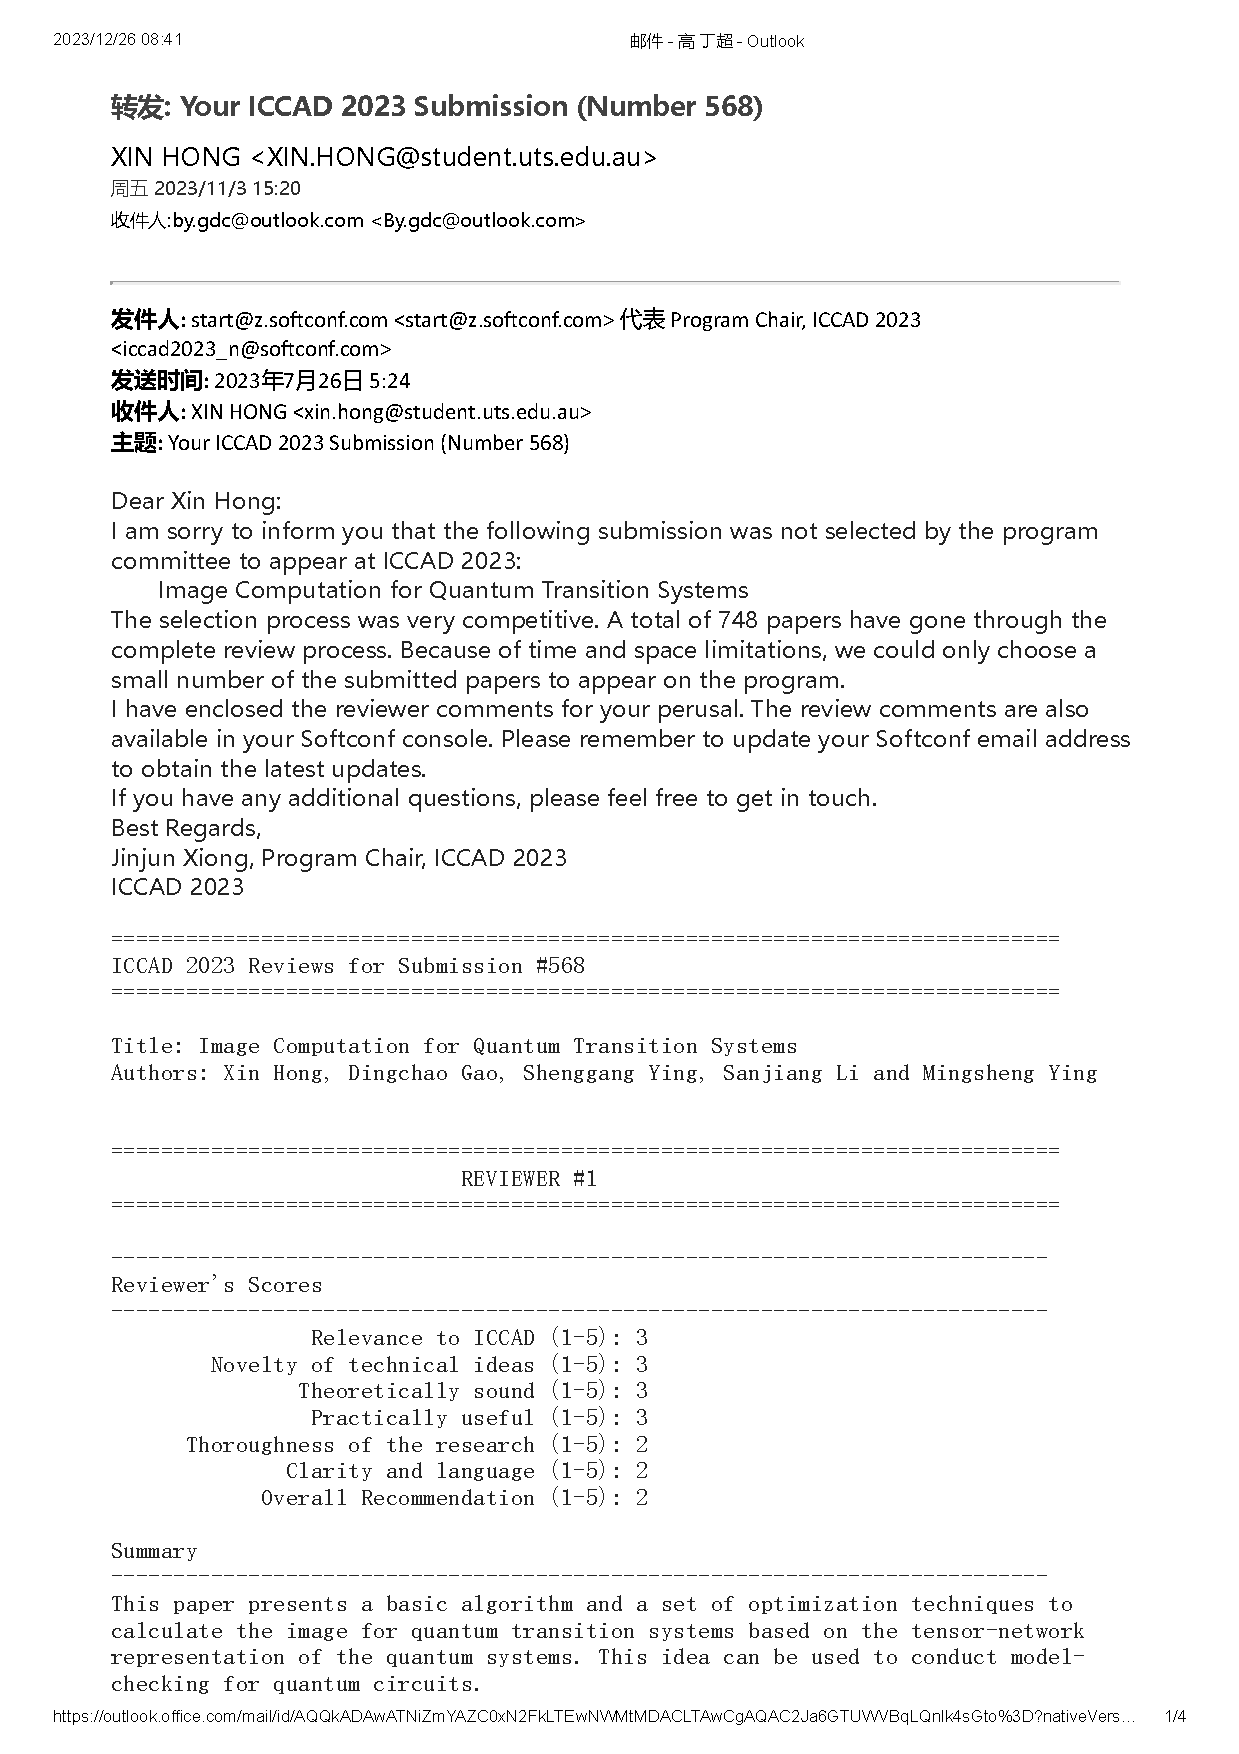
\includepdf[pages=1,scale = 0.8,pagecommand={\section*{附录一ICCAD审稿意见}}]{ICCAD.pdf}
% \includepdf[pages=2-,scale = 0.8]{ICCAD.pdf}
% 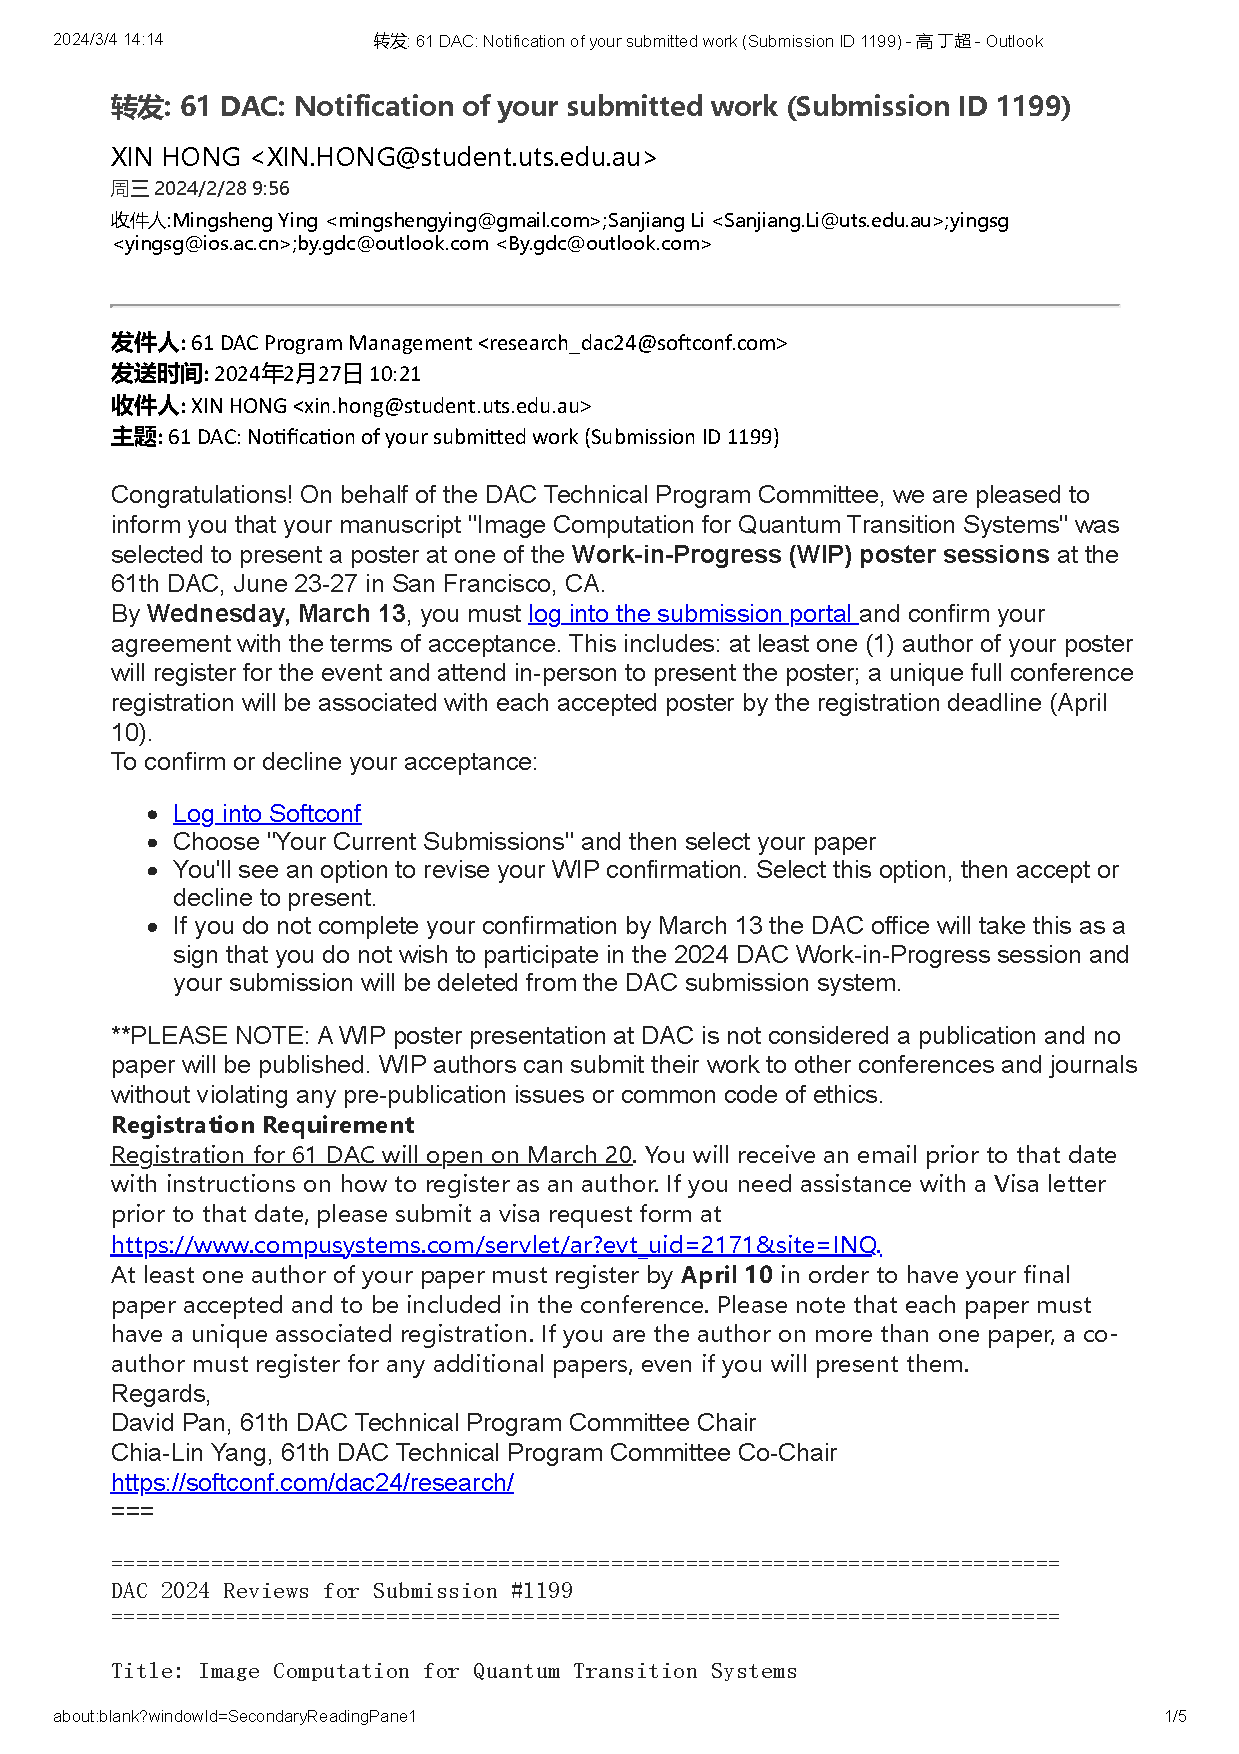
\includepdf[pages=1,scale = 0.8,pagecommand={\section*{附录二DAC审稿意见}}]{DAC.pdf}
% \includepdf[pages=2-,scale = 0.8]{DAC.pdf}
\end{document}
